\documentclass[40pt]{article}
\usepackage{ctex}
\usepackage{CJK}
\usepackage{graphicx}
\usepackage{picinpar,graphicx}
\usepackage{cite}
\usepackage{multirow}
\usepackage{hyperref,amsmath,amssymb,amscd}
\usepackage{geometry}
\setmainfont{Times New Roman}
\geometry{left=0.3cm,right=0.5cm,top=2.5cm,bottom=2.5cm}%Maybe it is the right choice.....
\usepackage{setspace}
\setlength{\parindent}{2em}
\twocolumn
\begin{document}
\title{\textbf{Reverse Connection with Objectness Prior Networks for Object Detection III}}
\author{\textbf{Liangjie Cao}}
\date{\textbf{21 May 2018}}
\maketitle
\par
\setlength{\baselineskip}{15pt}
\section{Training and Testing}
\textbf{In this section, the authors firstly introduce the multi-task loss function for optimizing the networks. And then they explain how to optimize the network jointly and perform inference directly. }
\begin{figure}[htbp]
 \centering
 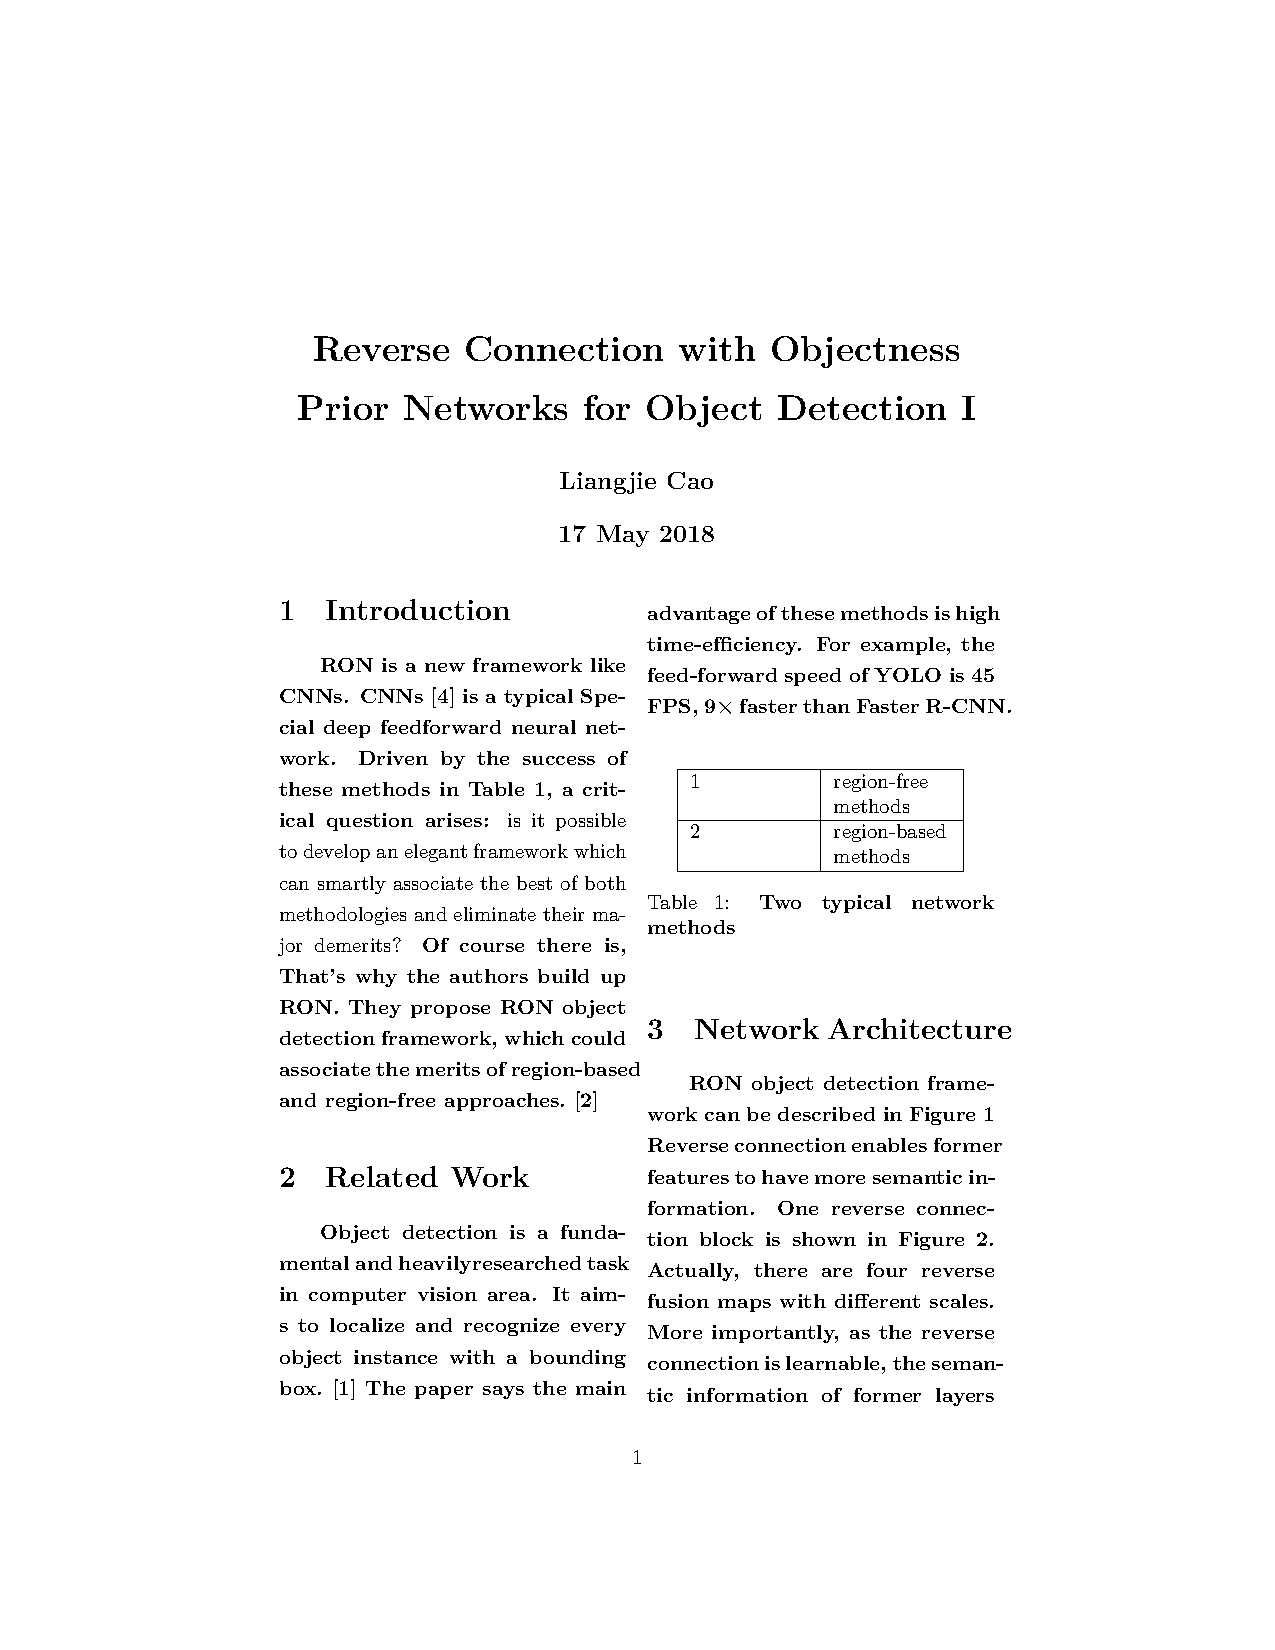
\includegraphics[width=0.5\textwidth]{RON.png}\\
 \caption{\textbf{RON object detection overview}}\label{Figure1}
 \end{figure}
\par
\section{Loss Function}
\textbf{They have three output branches. The first outputs the objectness confidence score $p ^{obj} = \{p ^{obj0}, p^{obj1\} }$, computed by a Softmax over the 2×A outputs of objectness prior (A = 10 in this paper, as there are 10 types of default boxes). The second branch outputs the boundingbox regression loss, denoted by Lloc. It targets at minimizing the smoothed L1 loss\cite{name1} between the predicted location offsets t = (tx,ty,tw,th) and the target offsets t1=(t1$_x$,t1$_y$,t1$_w$,t1$_h$). The third branch outputs the classification loss L$_{cls|obj}$ for each box, over K+1 categories. Then they use a multi-task loss L to jointly train the networks endto-end for objectness prior, classification and bounding-box regression:\\
 {\centering L=$\alpha$ $\frac{1}{N{obj}}$ L${_{obj}}$+ $\beta$ $\frac{1}{L{loc}}$ L${_{loc}}$+(1-$\alpha$-$\beta$)$\frac{1}{Nlcs|obj}$N${_{lcs|obj}}$ }
}
\par
\section{Joint Training and Testing}
\textbf{They optimize the models described above jointly with end-to-end training.At the beginning of training, the objectness prior maps are in chaos. However, along with the training progress, the objectness prior maps are more concentrated on areas covering objects.\cite{name2} Actually at training phase, each SGD mini-batch is constructed from N images chosen uniformly from the dataset. However, along with the training progress, the objectness prior maps are more concentrated on areas covering objects.
}\\
\section{Combining Objectness Prior with Detection}
\textbf{In this section, we explain how RON combines objectness prior with object detection. We assist object detection with objectness prior both in training and testing phases.And at the back-propagation phase, the network firstly generates the objectness prior, then for detection, samples whose objectness scores are high than threshold op are selected (Figure~\ref{Figure2}). Then Table~\ref{Table1} shows the result comparisons of the methods. I will continue learning in the following days.}
\footnote{Actually they note that the latest SSD uses new training tricks (color distortion, random expansion and online hard example mining), which makes the results much better. We expect these tricks will also improve our results, which is beyond the focus of this paper. }
\onecolumn \begin{table}[htbp]
 \begin{tabular}{p{1.5cm}|p{0.5cm}|p{0.5cm}p{0.5cm}p{0.5cm}p{0.5cm}p{0.5cm}p{0.5cm}p{0.5cm}p{0.5cm}p{0.5cm}p{0.5cm}p{0.5cm}p{0.5cm}p{0.5cm}p{0.5cm}p{0.5cm}p{0.5cm}p{0.5cm}p{0.5cm}p{0.5cm}p{0.5cm}}
    \hline
    Method & map & aero & bike & bird & boat & bottle & bus & car & cat & chair & cow & table & dog & horse & mbike & person & plant & sheep & sofa & train & tv \\
    \hline
    Fast R-CNN\cite{name1} & 70.0 & 77.0 & 78.1 & 69.3 & 59.4 & 38.3 & 81.6 & 78.6 & 86.7 & 42.8 & 78.8 & 68.9 & 84.7 & 82.0 & 76.6 & 69.9 & 31.8 & 70.1 & 74.8 & 80.4 & 70.4 \\
    Faster R-CNN\cite{name5} & 73.2 & 76.5 & 79.0 & 70.9 & 65.5 & 52.1 & 83.1 & 84.7 & 86.4 & 52.0 & \textbf{81.9} & 65.7 & 84.8 & 84.6 & 77.5 & 76.7 & 38.8 & 73.6 & 73.9 & 83.0 & 72.6 \\
    SSD300\cite{name4} & 72.1 & 75.2 & 79.8 & 70.5 & 62.5 & 41.3 & 81.1 & 80.8 & 86.4 & 51.5 & 74.3 & 72.3 & 83.5 & 84.6 & 80.6 & 74.5 & 46.0 & 71.4 & 73.8 & 83.0 & 69.1 \\
    SSD500\cite{name4} & 75.1 & 79.8 & 79.5 & 74.5 & 63.4 & 51.9 & 84.9 & \textbf{85.6} & 87.2 & 56.6 & 80.1 & 70.0 & 85.4 & 84.9 & 80.9 & 78.2 & 49.0 & \textbf{78.4} & 72.4 & 84.6  & 75.5   \\
    \hline
    RON320 & 74.2 & 75.7 & 79.4 & 74.8 & 66.1 & 53.2 & 83.7 & 83.6 & 85.8 & 55.8 & 79.5 & 69.5 & 84.5 & 81.7 & 83.1 & 76.1 & 49.2 & 73.8 & 75.2 & 80.3 & 72.5 \\
    RON384 & 75.4 & 78.0 & 82.4 & 76.7 & 67.1 & 56.9 & 85.3 & 84.3 & 86.1 & 55.5 & 80.6 & 71.4 & 84.7 & 84.8 & 82.4 & 76.2 & 47.9 & 75.3 & 74.1 & 83.8 & 74.5 \\
    RON320++ & 76.6 & 79.4 & \textbf{84.3} & 75.5 & 69.5 & 56.9 & 83.7 & 84.0 & 87.4 & 57.9 & 81.3 & 74.1 & 84.1 & 85.3 & 83.5 & 77.8 & 49.2 & 76.7 & 77.3 & 86.7 & 77.2 \\
    RON384++ & \textbf{77.6} & 86.0 & 82.5 & 76.9 & 69.1 & 59.2 & 86.2 & 85.5 & 87.2 & 59.9 & 81.4 & 73.3 & 85.9 & 86.8 & 82.2 & 79.6 & 52.4 & 78.2 & 76.0 & 86.2 & 78.0 \\
  \end{tabular}
  \caption{\textbf{Detection results on PASCAL VOC 2007 test set. The entries with the best APs for each object category are bold-faced.}} \label{Table1}
  \end{table}
\begin{figure}[htbp]
  \centering
 \includegraphics[width=0.5\textwidth]{map.png}\\
 \caption{\textbf{Mapping the objectness prior with object detection}}\label{Figure2}
\end{figure}
\twocolumn \bibliographystyle{plain}
\bibliography{yinyong1}
\end{document}

